\documentclass{scrarticle}
\usepackage[a4paper, total={6in, 10in}]{geometry}
\usepackage[ngerman]{babel}

\usepackage{xcolor}
\usepackage{graphicx}
\usepackage{multirow} % Wichtig: Fügen Sie dieses Paket in Ihrer Präambel hinzu!
\usepackage{array} % Oft nützlich in Verbindung mit tabularx

\usepackage{amsmath}
\usepackage{amsthm}
\usepackage{amssymb}
\usepackage{algorithm}
\usepackage[noend]{algpseudocode}

\usepackage{tikz}

\usepackage[colorlinks=true, linkcolor=black, citecolor=black, urlcolor=black]{hyperref}

\newtheorem{satz}{Satz}[section]
\newtheorem{lemma}{Lemma}[section]
\newtheorem{definition}{Definiton}[section]
\numberwithin{equation}{section}

\makeatletter
\renewcommand{\ALG@name}{Algorithmus}
\makeatother
\algrenewcommand\algorithmicrequire{\textbf{Eingabe:}}
\algrenewcommand\algorithmicensure{\textbf{Ausgabe:}}

\title{Metal-Oxide-Semiconductor-Transistoren}
\author{Stephan Epp\\\texttt{hjstephan86@gmail.com}}
\date{\today}

\begin{document}
	\maketitle
	\vspace{5em}
	\tableofcontents
	\newpage

\section{Einleitung}
Die Grundlage hochintegrierter Schaltungen bilden heute Metal-Oxide-Semiconductor-Tran-sistoren (MOS-Transistoren). Es gibt pMOS-Transistoren und nMOS-Transistoren. Zum Beispiel bezieht sich das n vor MOS dabei auf das Substrat des nMOS-Transistors. Der nMOS-Transistor besteht aus einem n-p-n-Übergang, bei dem ein leitender Zustand nur dann erfolgt, wenn Elektronen als Minoritätsladungsträger im p-Substrat durch den Feldeffekt unter den Metall-Oxid-Isolator gezogen werden.

Die U-I-Kennlinie eines nMOS-Transistors folgt in den verschiedenen Betriebsbereichen spezifischen mathematischen Formeln. Diese Formeln basieren auf physikalischen Modellen des Transistors und beschreiben den Drain-Source-Strom $I_{DS}$ in Abhängigkeit von den angelegten Spannungen. Diese bestehen hauptsächlich aus der Gate-Source-Spannung $U_{GS}$ und der Drain-Source-Spannung $U_{DS}$. Es gibt drei Betriebsbereiche für einen nMOS-Transistor: den Sperrbereich, den Triodenbereich und den Sättigungsbereich.

\section{nMOS-Transistor}
In diesem Kapitel werden die drei Betriebsbereiche eines nMOS-Transistors beschrieben.
\subsection{Sperrbereich}
In diesem Bereich ist der Transistor ausgeschaltet und leitet praktisch keinen Strom.

\begin{enumerate}
	\renewcommand{\labelenumi}{} % Keine Nummerierung
	\item \textbf{Bedingung}: $U_{GS} < U_{TH}$, wobei $U_{TH}$ die Schwellenspannung ist.
	\item \textbf{Formel}:
	\begin{equation*}
		I_{DS} \approx 0
	\end{equation*}
	\item \textbf{Erklärung}: Wenn die Gate-Source-Spannung $U_{GS}$ unter der Schwellenspannung $U_{TH}$ liegt, kann sich kein leitender Kanal zwischen Source und Drain bilden, und es fließt kein nennenswerter Strom, d.h., $I_{DS} \approx 0$. Idealisiert ist $I_{DS} = 0$, in der Realität gibt es einen sehr kleinen Leckstrom (Subthreshold-Strom), der oft vernachlässigt wird.
\end{enumerate}

\subsection{Triodenbereich / Linearer Bereich}
Dieser Bereich wird auch als ohmscher Bereich bezeichnet, da der Transistor hier wie ein spannungsgesteuerter Widerstand wirkt. Der Strom steigt hier nahezu linear mit $U_{DS}$ an (für kleine $U_{DS}$) und ist stark von $U_{GS}$ abhängig.

\begin{enumerate}
	\renewcommand{\labelenumi}{} % Keine Nummerierung
	\item \textbf{Bedingung}: $U_{GS} > U_{TH}$ und $U_{DS} < (U_{GS} - U_{TH})$
	\item \textbf{Formel} bei vereinfachtem Modell für lange Kanäle:
	\begin{equation*}
		I_{DS} = \mu_n C_{ox} \frac{W}{L} \left( (U_{GS} - U_{TH})U_{DS} - \frac{1}{2}U_{DS}^2 \right)
	\end{equation*}
	\begin{itemize}
		\item[-] $\mu_n$: Elektronenbeweglichkeit im Kanal
		\item[-] $C_{ox}$: Oxidkapazität pro Flächeneinheit
		\item[-] $W$: Kanalbreite
		\item[-] $L$: Kanallänge
		\item[-] $U_{TH}$: Schwellenspannung
	\end{itemize}
	\item \textbf{Erklärung}: Wenn die Gate-Spannung $U_{GS}$ größer als die Schwellenspannung $U_{TH}$ ist, entsteht ein leitender Kanal im Transistor. Solange die Drain-Spannung $U_{DS}$ nicht zu hoch ist, verhält sich der Kanal wie ein variabler Widerstand. Der Strom steigt an, wenn $U_{DS}$ zunimmt. Dabei wird der Kanal zum Drain hin etwas schmaler. Dies führt zu einer nicht-linearen Beziehung zwischen Strom und Spannung, die durch den Term $U_{DS}^2$ beschrieben wird. Der nicht-lineare Anstieg beschreibt, wie der Strom vom gesperrten Zustand in den leitenden Zustand übergeht, bevor er schließlich in die Sättigung geht.
\end{enumerate}

\subsection{Sättigungsbereich}
In diesem Bereich verhält sich der Transistor wie eine spannungsgesteuerte Stromquelle, da der Drain-Source-Strom weitgehend unabhängig von $U_{DS}$ ist.

\begin{enumerate}
	\renewcommand{\labelenumi}{} % Keine Nummerierung
	\item \textbf{Bedingung}: $U_{GS} > U_{TH}$ und $U_{DS} \ge (U_{GS} - U_{TH})$
	\item \textbf{Formel} bei vereinfachtem Modell für lange Kanäle:
	\begin{equation*}
		I_{DS} = \frac{1}{2} \mu_n C_{ox} \frac{W}{L} (U_{GS} - U_{TH})^2 \left( 1 + \lambda U_{DS} \right)
	\end{equation*}
		\item Der Term $(1 + \lambda U_{DS})$ berücksichtigt den \textbf{Kanallängenmodulationseffekt}, $\lambda$ ist der Kanallängenmodulationsparameter, der eine leichte Zunahme des Stroms mit $U_{DS}$ in der Sättigung beschreibt. Ohne diesen Effekt wäre der Strom konstant.
	\item \textbf{Erklärung}: Sobald $U_{DS}$ einen bestimmten Wert erreicht ($U_{DS,sat} = U_{GS} - U_{TH}$), wird der Kanal am Drain-Ende abgeschnürt (pinch-off). Eine weitere Erhöhung von $U_{DS}$ führt nicht zu einer signifikanten Zunahme des Stroms, da der Stromfluss durch die Anzahl der Ladungsträger im Kanal und die Gate-Spannung begrenzt wird.
\end{enumerate}

\subsection{U-I-Kennlinie für $U_{GS} = 2\,\mathrm{V}$}

Für \( U_{GS} = 2\,\mathrm{V} \), \( U_{TH} = 0.2\,\mathrm{V} \) und \( k = 1\,\mathrm{mA/V^2} \) ergibt sich:
\begin{figure}[h]
	\centering
	\label{fig:kennlinie}
	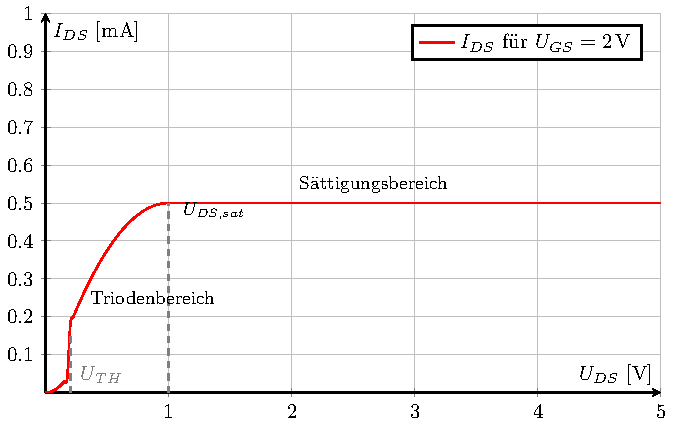
\includegraphics[scale=1.0]{tkiz/ui-kennlinie.pdf}
	\caption{Idealisierte U-I-Kennlinie eines nMOS-Transistors mit $U_{GS} = 2\,\mathrm{V}$}
\end{figure}
\begin{enumerate}
	\renewcommand{\labelenumi}{} % Keine Nummerierung
	\item \textbf{Sperrbereich}: $U_{GS} < U_{TH}$, näherungsweise $U_{DS} < 0.2\,\mathrm{V}$ \\
	\[
	I_{DS} \approx 0\,\mathrm{mA}
	\]
	\item \textbf{Triodenbereich}: $U_{TH} < U_{DS} < (U_{GS} - U_{TH})$, d.h., $0.2\,\mathrm{V} < U_{DS} < 1.8\,\mathrm{V}$ \\
	\[
	I_{DS} = k \left((U_{GS} - U_{TH}) U_{DS} - \frac{1}{2} U_{DS}^2\right)
	\]
	\item \textbf{Sättigungsbereich}: $U_{DS} \ge (U_{GS} - U_{TH}) = U_{DS,sat}$, d.h., $U_{DS} \ge 1.8\,\mathrm{V}$ \\
	\[
	I_{DS} = \frac{1}{2} k (U_{GS} - U_{TH})^2 = 1,62\,\mathrm{mA}
	\]
\end{enumerate}

\section{Complementary Metal-Oxide-Semiconductor (CMOS)}
\label{sec:cmos}
Bevor der CMOS Schaltkreis betrachtet wird, wird das Schaltsymbol des pMOS-Transistors und das Schaltsymbol des nMOS-Transistors in Abbildung \ref{fig:pmos-nmos} gezeigt.
\begin{figure}[ht]
	\centering
	\begin{minipage}[t]{0.45\textwidth}
		\centering
		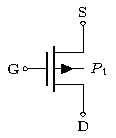
\includegraphics[scale=2.2]{tkiz/pmos.pdf}
	\end{minipage}
	\hfill
	\begin{minipage}[t]{0.45\textwidth}
		\centering
		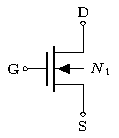
\includegraphics[scale=2.2]{tkiz/nmos.pdf}
	\end{minipage}
	\caption{Schaltsymbol des pMOS-Transistors $P_1$ und des nMOS-Transistors $N_1$}
	\label{fig:pmos-nmos}
\end{figure}

Complementary Metal-Oxide-Semiconductor (CMOS) Schaltkreise sind Schaltkreise, in denen der pMOS- und der nMOS-Transistor komplementär zueinander verbunden werden.
\begin{figure}[h]
	\centering
	\label{fig:cmos-not}
	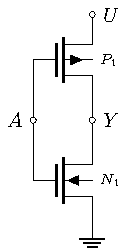
\includegraphics[scale=1.7]{tkiz/cmos-not.pdf}
	\caption{CMOS-Schaltung}
\end{figure}
Abbildung \ref*{fig:cmos-not} zeigt eine CMOS-Schaltung mit der Betriebsspannung $U$, der Eingangsspannung $A$ für die Transistoren $P_1$ und $N_1$ und der Ausgangsspannung $Y$. Dabei ist $P_1$ der pMOS-Transistor und $N_1$ der nMOS-Transistor.

Beim nMOS-Transistor $N_1$ zeigt der Pfeil auf den Transistor. Dies zeigt seine physikalische Wirkungsweise. Ist die Eingangsspannung $A$ ausreichend groß, dann liegt am Gate eine positive Spannung an. Das bewirkt wie beim Kondensator einen Feldeffekt zwischen der Oberfläche der Metall-Elektrode mit positiven Ladungsträgern und der Unterkante des Metall-Oxid-Isolators mit negativen Ladungsträgern. Dieser Feldeffekt zieht die Minoritätsladungsträger (Elektronen) im p-Substrat des nMOS-Transistors unter den Metall-Oxid-Isolator. Erst durch diesen Feldeffekt tragen die Minoritätsladungsträger in ihrer Unterzahl im p-Substrat zum Stromfluss bei. Es entsteht ein leitender Kanal von Elektronen. Ist die Eingangspannung nämlich nicht ausreichend hoch, sperrt der nMOS-Transistor. Daher wird der nMOS-Transistor auch nMOS-Feldeffekttransistor (nMOSFET) genannt.

Beim pMOS-Transistor $P_1$ zeigt der Pfeil weg vom Transistor. Das liegt daran, dass die Elektronen im pMOS-Transistor nicht Minoritätsladungsträger sondern Majoritätsladungs-träger im n-Substrat sind. Das heißt, der pMOS-Transistor leitet sogar schon bei einer Eingangsspannung von $A = 0\mathrm{V}$. Der Feldeffekt beim pMOS-Transistor führt dazu, dass bei ausreichender Eingangsspannung $A$ am Gate die Minoritätsladungsträger im n-Substrat unter den Metall-Oxid-Isolator gezogen werden und der pMOS-Transistor sperrt. Daher wird der pMOS-Transistor auch pMOS-Feldeffekttransistor (pMOSFET) genannt.

Beide Transistoren $P_1$ und $N_1$ in Reihe geschaltet haben somit ein physikalisch komplementäres Sperr- und Leitverhalten zueinander. Dieses komplementäre Sperr- und Leitverhalten gibt diesem Schaltkreis den Namen Complementary Metal-Oxide-Semiconductor (CMOS) Schaltkreis.

Betrachtet man das logische Schaltverhalten der CMOS Schaltung in Abhängigkeit der Betriebsspannung $U$, der Eingangsspannung $A$ und der Ausgangsspannung $Y$, wird klar, dass mit dieser Schaltung ein Inverter betrieben wird. Ist $A = 0$, leitet $P_1$ und $N_1$ sperrt. Das heißt, das Bezugspotenzial für $Y$ ist $U$ und damit ist $Y = 1$ (Pull-Up-Bezugspotenzial). Ist $A = 1$, sperrt $P_1$ und $N_1$ leitet. Das heißt, das Bezugspotenzial für $Y$ ist die Masse und damit ist $Y = 0$ (Pull-Down-Bezugspotenzial).

\section{Logische Gatter: NND und NOR}
Ein logisches Gatter (oft auch einfach Gatter oder englisch (logic) gate genannt) ist ein grundlegender Baustein in der digitalen Elektronik, der eine bestimmte boolesche Funktion berechnet.
\begin{figure}[ht]
	\begin{minipage}[t]{0.5\textwidth}
		\centering
		\begin{tabular}{c|c||c}
			\hline
			$A$ & $B$ & $A \text{ NND } B$ \\
			\hline\hline
			0 & 0 & 1 \\
			0 & 1 & 1 \\
			1 & 0 & 1 \\
			1 & 1 & 0 \\
			\hline
		\end{tabular}
	\end{minipage}
	\hfill % Sorgt für horizontalen Abstand zwischen den minipages
	\begin{minipage}[t]{0.5\textwidth}
		\centering
		\begin{tabular}{c|c||c}
			\hline
			$A$ & $B$ & $A \text{ NOR } B$ \\
			\hline\hline
			0 & 0 & 1 \\
			0 & 1 & 0 \\
			1 & 0 & 0 \\
			1 & 1 & 0 \\
			\hline
		\end{tabular}
	\end{minipage}
	\caption{Boolesche Funktion NND und NOR}
\label{fig:nand-nor}
\end{figure}
In Kapitel \ref{sec:cmos} wird ein Inverter beschrieben, der die boolesche Funktion des NOT Gatters in Abhängigkeit des Eingangssignals $A$ berechnet. Andere Gatter, die durch CMOS-Schaltungen gebildet werden können, sind das NAND (kurz: NND) Gatter und das NOR Gatter. Das NND Gatter und das NOR Gatter bilden boolesche Funktionen in Abhängigkeit der Eingangssignale $A$ und $B$. Abbildung \ref{fig:nand-nor} zeigt die vollständig beschriebene boolesche Funktion beider Gatter. Dadurch, dass diese booleschen Funktionen durch MOSFETs gebildet werden können, sind ihre Funktionen als Hardwarelösung nutzbar. Das bedeutet, der Prozessor kann diese Funktion ohne ein geschriebenes Programm direkt in der Hardware auswerten.

Wie lange braucht der Prozessor dafür? Der Takt eines Prozessors ist die kleinste Zeiteinheit, in der der Prozessor periodisch einen Arbeitsschritt ausführt. Die kleinste Zeiteinheit wird aber deutlicher beschrieben durch den Begriff \textit{Slot}, da Slot die dem Prozessor zur Verfügung stehende Zeit betont. Der Vorteil von in Hardware nutzbaren Funktionen ist der, dass der Prozessor in einem Slot z.B. die Ergebnisse der NND Funktion oder der NOR Funktion auswerten kann. Würde der Prozessor z.B. für die NND Funktion ein geschriebenes Programm ausführen, könnte er mit dieser Programmausführung die NND Funktion nicht in einem Slot auswerten.

Es ist zu beachten, dass die NND Funktion oder die NOR Funktion mit der einfachen Realisierung durch MOSFETs jeweils in einem Slot vom Prozessor ausgewertet werden kann. Diese Funktionen gehören zu den grundlegenden Hardwarefunktionen eines Prozessors. Es gibt komplexere Funkionen, die auch durch elektronische Schaltungen in Hardware realisiert werden. Diese Funktionen aber kann der Prozessor nicht in einem Slot auswerten, benötigt dafür aber immer noch weit weniger Slots als wenn er sie durch ein geschriebenes Programm auswerten müsste. Andererseits ist es nicht so, dass deshalb jede komplexere Funktion in Hardware gelöst wird. Der Grund dafür ist, dass der Aufwand bzw. die Kosten und der Nutzen unverhältnismäßig sind im Vergleich dazu, dass die komplexeren Funktionen in einem geschriebenen Programmen ausgewertet werden. Die komplexen Funktionen sind heute so groß und ändern sich so häufig, dass es generische Microcontroller braucht, die programmierbar sind mit geschriebenen Programmen. Diese komplexen Funktionen werden von eingebetteten Systemen ausgeführt wie z.B. die Auswertung von Radarobjekten in der Automobilindustrie.

\section{Eingebettetes System}
Ein eingebettetes System ist eine Hardware-/Software-Einheit, die innerhalb einer physikalischen Umgebung Aufgaben in Echtzeit bearbeitet. Die Aufgaben oder Tasks haben harte Deadlines und müssen vom Prozessor so ausgeführt werden, dass alle Deadlines eingehalten werden. Eine harte Deadline darf auf keinen Fall überschritten werden. Beispiele für physikalische Umgebungen, in denen eingebettete Systeme heute eingebettet sind, sind Flugzeuge, Züge, Autos oder Smartphones.

\subsection{Scheduling}
Damit alle Tasks in einer geplanten und geordneten Reihenfolge ausgeführt werden können, gibt es den Scheduler, der den Schedule für alle Tasks plant. An diesen Schedule hält sich der Prozessor zur Bearbeitung aller Aufgaben, da erst so das Einhalten aller Deadlines \textit{garantiert} wird.

Earliest Deadline First (EDF) ist eine Vorgehensweise zur Scheduleberechnung, bei der die Menge an Tasks \textit{vorher bekannt} ist. Nach EDF wird die Menge an Tasks gierig nach Deadlines sortiert und entsprechend priorisiert. Je früher die Deadline einer Task ist, desto höher ist ihre Priorität und desto früher wird sie ausgeführt. Es kann passieren, dass während der Ausführung des Schedules eine Task blockiert, da sie auf eine Ressource warten muss. Die Idee von EDF$^+$ ist, dass Tasks, die blockieren, mit geringster Priorität bestraft werden und anschließend der EDF Schedulue so schnell wie möglich neu berechnet und dann ausgeführt wird.
\begin{satz}
	\label{satz:edf+}
	EDF$^+$ ist optimal in der Garantieaussage über die gesamte Zeit, in der Tasks ausgeführt werden.
\end{satz}
\begin{proof}
	EDF ist optimal in der Auslastung des Prozessors. Dies ist eine Garantieaussage. Sobald eine Task verdrängt werden muss, weil sie blockiert und auf eine andere Ressource wartet, und damit vom optimalen Schedule abgewichen werden muss, ist die Garantieaussage verletzt. Das heißt, es muss dann so schnell wie möglich die Garantieaussage wiederhergestellt werden. Dazu wird die Task, die blockiert hat, mit niedrigster Priorität bestraft. Anschließend wird EDF zur Scheduleberechnung ausgeführt und dieser neue Schedule mit der Garantieaussage für alle Tasks zur Bearbeitung genutzt. Es muss ein neuer Schedule berechnet werden, da die Garantieaussage des alten Schedules mit neuer Priorisierung der blockierten Task verletzt wurde. Dieses Vorgehen ist optimal hinsichtlich der Zeit der Ausführung des Schedules, über die eine Garantieaussage des optimalen EDF Schedules gemacht wird. Denn das Risiko, dass die blockierte Task noch einmal blockiert, wird dadurch minimiert, dass sie, weil sie blockiert hat, die niedrigste Priorität erhält.
\end{proof}
Es ist zu beachten, dass es während der Ausführung von Tasks, die nach dem EDF$^+$ Schedulue ausgeführt werden, immer wieder zu Unterbrechungen kommen kann, wenn das Nutzen anderer Ressourcen nicht möglich ist. Das heißt, die Anzahl der Unterbrechungen sind vorher nicht bekannt und können dazu führen, dass einige Tasks aus der Menge aller Tasks \textit{nicht} bis zu ihrer Deadline ausgeführt werden können.

Was kann dazu führen, dass eine Task während der Ausführung des Schedules blockiert? Tasks könnten einen kritischen Abschnitt betreten oder auf gemeinsam genutzten Speicher zugreifen. Wird die geometrisch verteilte Zufallsvariable $X$ betrachtet, die die Anzahl der Versuche bis zur ersten blockierten Task zählt und mit $p$ die Wahrscheinlichkeit, dass eine Task blockiert, dann ist der Erwartungswert $E(X)$ gegeben durch $E(X)= 1 / p$. Der konkrete Wert für $p$ ist so nicht einfach zu bestimmen. Ist z.B. $p = 0.1$, dann ist $E(X) = 10$, d.h., die ersten 10 Tasks blockieren nicht und erst die 11. Task blockiert.
\begin{table}[h]
	\centering
	\begin{tabular}{m{3.5cm}|m{3.5cm}|m{3.5cm}}
		\hline
		Wahrscheinlichkeit $p$ & Erwartungswert $1/p$ & Blockierte Tasks\\
		\hline\hline
		0.05 & 20.00 & 2.00 \\
		0.10 & 10.00 & 4.00 \\
		0.15 & 6.67 & 6.00 \\
		0.20 & 5.00 & 8.00 \\
		0.25 & 4.00 & 10.00 \\
		0.30 & 3.33 & 12.00 \\
		0.35 & 2.86 & 14.00 \\
		0.40 & 2.50 & 16.00 \\
		0.45 & 2.22 & 18.00 \\
		0.50 & 2.00 & 20.00 \\
		\hline
	\end{tabular}
	\caption{Erwartete Anzahl blockierter Tasks bei 40 Tasks}
	\label{tab:geometric-expectation}
\end{table}
Tabelle \ref{tab:geometric-expectation} zeigt für jede Zeile in der rechten Spalte die erwartete Anzahl blockierter Tasks, wenn davon ausgegangen wird, dass 40 Tasks ausgeführt werden. Blockiert eine Task mit der Wahrscheinlichkeit $p = 0.05$, dann gibt es im Mittel 2 Tasks, die blockieren. Ist $n$ die Anzahl der Tasks, benötigt das Berechnen eines neuen Schedules nach EDF$^+$ mit Merge-Sort eine Laufzeit von $O(n \log(n))$. Da Merge-Sort nach dem optimalen Teile-und-Herrsche Prinzip die Tasks nach ihren Prioritäten sortiert, ist die Berechnung eines neuen Schedules nicht schneller möglich. 

Die Garantieaussage von EDF$+$ in Satz \ref{satz:edf+} hält auch für \textit{wachsende Taskmengen}, wo Tasks während der Ausführung des Schedules zur Taskmenge hinzugefügt werden. Je nach Deadline der neuen Task wird sie dann in der spontanen Neuberechnung des Schedules berücksichtigt und ggf. sogar als erste Task ausgeführt und beendet.


\section{Software Engineering}
Software Engineering ist die Disziplin, bei der Ingenieure für das Softwareprodukt ihr Fachwissen so einbringen, dass alle Anforderungen an die Software unter möglichst allen Umstän-den erfüllt werden. Das heißt, zu jeder Zeit und unabhängig von ihrer Auslastung und Umgebung muss die Software alle Prozessanfragen aller Benutzer bearbeiten entsprechend der spezifizierten Anforderungen. Erst so wird den Benutzern mit der Software ermöglicht, Aufgaben und Abläufe zu bearbeiten. Wichtige Anforderungen an die Software sind z.B. die Benutzerfreundlichkeit, Zuverlässigkeit und Robustheit. Zur Benutzerfreundlichkeit zählen zum Beispiel einfache und intuitive Bedienung der Software und die Effizienz.

\textbf{Um alle diese Anforderungen zu erfüllen, ist ein \textit{standardisierter Entwicklungsprozess für Software} nötig}. Alle beteiligten Ingenieure, die die Software entwickeln, Produktmanager und Benutzer müssen diesen standardisierten Entwicklungsprozess kennen und diszipliniert leben. Nur so kann die Qualität im Entwicklungsprozess, egal in welcher Entwicklungsphase, sichergestellt werden. Die Qualität des Entwicklungsprozesses hat einen sehr hohen Einfluss auf die Qualität der Software selbst. Mit den Anforderungen aus Benutzersicht werden auch Anforderungen an die Software gestellt wie Analysierbarkeit, Erweiterbarkeit und Wartbarkeit. Ingenieure, die nach dem standardisierten Entwicklungsprozess Software entwickeln, sind damit entlastet, weil so alle Beteiligten wie Benutzer und Produktmanager berücksichtigen, dass spontane Änderungen an die Software \textit{nur und immer} nach dem Standard umzusetzen sind.

Der standardisierte Entwicklungsprozess muss agil sein und dem V-Model entsprechen. Agil bedeutet, dass Releases eine Dauer von maximal 5 bis 6 Wochen haben. Zudem helfen regelmäßige Stand-Ups und eine spontane Meeting Kultur, bei der ein Meeting möglichst nicht länger als eine halbe Stunde dauern und an dem möglichst nur 2 bis höchstens 3 Personen teilnehmen sollten. Die spontane Meeting Kultur ist wichtig, weil damit jedem Ingenieur zu jeder Zeit das Vertrauen in das Team bei schwierigen Fragen gestärkt wird und mit der Hilfe anderer Teamkollegen in kurzer Zeit zu rechnen ist. V-Model bedeutet, dass zur Entwicklung auf allen Ebenen auch die Qualitätssicherung durchgeführt werden muss. Bei der Qualitätssicherung helfen automatisierte Tests wie Unit Tests, Integrationstests und Benutzertests. Es kann wichtig sein, auch manuelle Benutzertests durchzuführen.

\textit{Integrationstests getrieben durch zyklomatische Komplexität} bedeutet, dass Ingenieure mit Hilfe der Testabdeckung durch Integrationstests das Refactoring da beginnen, wo die zyklomatische Komplexität am höchsten ist. Die Idee ist, dass mit der Ausführung der Integrationstests auch der Coverage Report für jede Klasse und Methode ausgewertet wird. Der Coverage Report enthält die zyklomatische Komplexität, welche für alle Klassen und Methoden ausgelesen und in eine Textdatei \textit{cc.txt} geschrieben und in Git versioniert wird. Dabei enthält cc.txt alle Klassen und Methoden absteigend sortiert. So sieht jeder Ingenieur leicht, für welche Klassen und Methoden das Refactoring anzuwenden ist und durch welches Refactoring in der Vergangenheit die zyklomatische Komplexität wie reduziert wurde.

\section{Zusammenfassung}
Zunächst werden die nMOS-Transistoren detailliert beschrieben. Dabei wird die Funktionsweise anhand der U-I-Kennlinie in ihren drei Betriebsbereichen -- dem Sperrbereich, Triodenbereich (linearer Bereich) und Sättigungsbereich -- erläutert. Die jeweiligen Bedingungen und zugehörigen mathematischen Formeln für den Drain-Source-Strom ($I_{DS}$) werden präsentiert und durch eine idealisierte U-I-Kennlinie visuell dargestellt. Physikalische Effekte wie die Kanallängenmodulation werden berücksichtigt.

Im Anschluss wird die Complementary Metal-Oxide-Semiconductor (CMOS)-Technologie behandelt. Die komplementäre Funktionsweise von pMOS- und nMOS-Transistoren wird anhand ihrer Schaltsymbole und ihres spezifischen Sperr- und Leitverhaltens erklärt. Die Implementierung eines CMOS-Inverters wird als grundlegendes Beispiel für die Nutzung dieser Technologie zur Realisierung boolescher Funktionen dargelegt.

Weiterhin werden logische Gatter wie das NAND (NND) und NOR Gatter thematisiert. Ihre booleschen Funktionen werden in Wahrheitstabellen dargestellt. Es wird erläutert, dass diese Gatter als Hardwarelösungen in Prozessoren implementiert werden können, was eine schnellere Verarbeitung in einem Prozessor-Slot ermöglicht, im Gegensatz zur Ausführung durch Softwareprogramme. Die Abwägung zwischen Hardware- und Softwarelösungen für komplexere Funktionen, insbesondere im Kontext von Microcontrollern und eingebetteten Systemen, wird diskutiert.

Ein separater Abschnitt widmet sich den eingebetteten Systemen, die als Hardware-/Software Einheiten Aufgaben in Echtzeit mit harten Deadlines ausführen. Das Scheduling von Tasks wird als essenzieller Bestandteil solcher Systeme hervorgehoben. Besonders wird das Earliest Deadline First (EDF)-Verfahren beschrieben und die Erweiterung EDF$^+$ vorgestellt, welche unter Berücksichtigung blockierender Tasks EDF optimal erweitert. Die Garantieaussage von EDF$+$ hält auch für wachsende Taskmengen, wo Tasks während der Ausführung des Schedules zur Taskmenge hinzugefügt werden. Durch die spontane Neuberechnung macht es Sinn, zu untersuchen, in wie weit EDF$+$ auch für das Scheduling in Betriebssystem wie z.B. Linux verwendet werden kann. Harte Deadlines müssen auf jeden Fall eingehalten werden. Beim Überschreiten von weichen Deadlines degegen hat das Betriebssystem noch keine sicherheitskritische Grenze überschritten, die lebensbedrohliche Folgen für den Anwender und seine Umgebung hat. 

Abschließend wird der Bereich des Software Engineerings beleuchtet. Es wird betont, dass ein standardisierter, agiler Entwicklungsprozess erforderlich ist, um Qualitätsanforderungen wie Benutzerfreundlichkeit, Zuverlässigkeit, Robustheit, Analysierbarkeit, Erweiterbarkeit und Wartbarkeit zu erfüllen. Die Bedeutung von kurzen Release-Zyklen, regelmäßigen Stand-Ups und einer spontanen Meeting-Kultur im agilen Kontext wird unterstrichen. Des Weiteren wird die Relevanz des V-Modells für die Qualitätssicherung auf allen Ebenen, insbesondere durch automatisierte Tests (Unit-, Integrations- und Benutzertests), herausgestellt. Ein spezifischer Ansatz, bei dem Integrationstests durch zyklomatische Komplexität getrieben werden, wird beschrieben, um Refactoring-Bedarfe zu identifizieren und die Code-Qualität kontinuierlich zu verbessern.

\end{document}